\documentclass[border=10pt]{standalone}
\usepackage[svgnames]{xcolor}
\usepackage{amsmath}
\usepackage{pgfplots}
\pgfplotsset{compat=newest}
\usepackage[sfdefault]{FiraSans}
\usepackage{FiraMono}
\renewcommand*\familydefault{\sfdefault}
\begin{document}
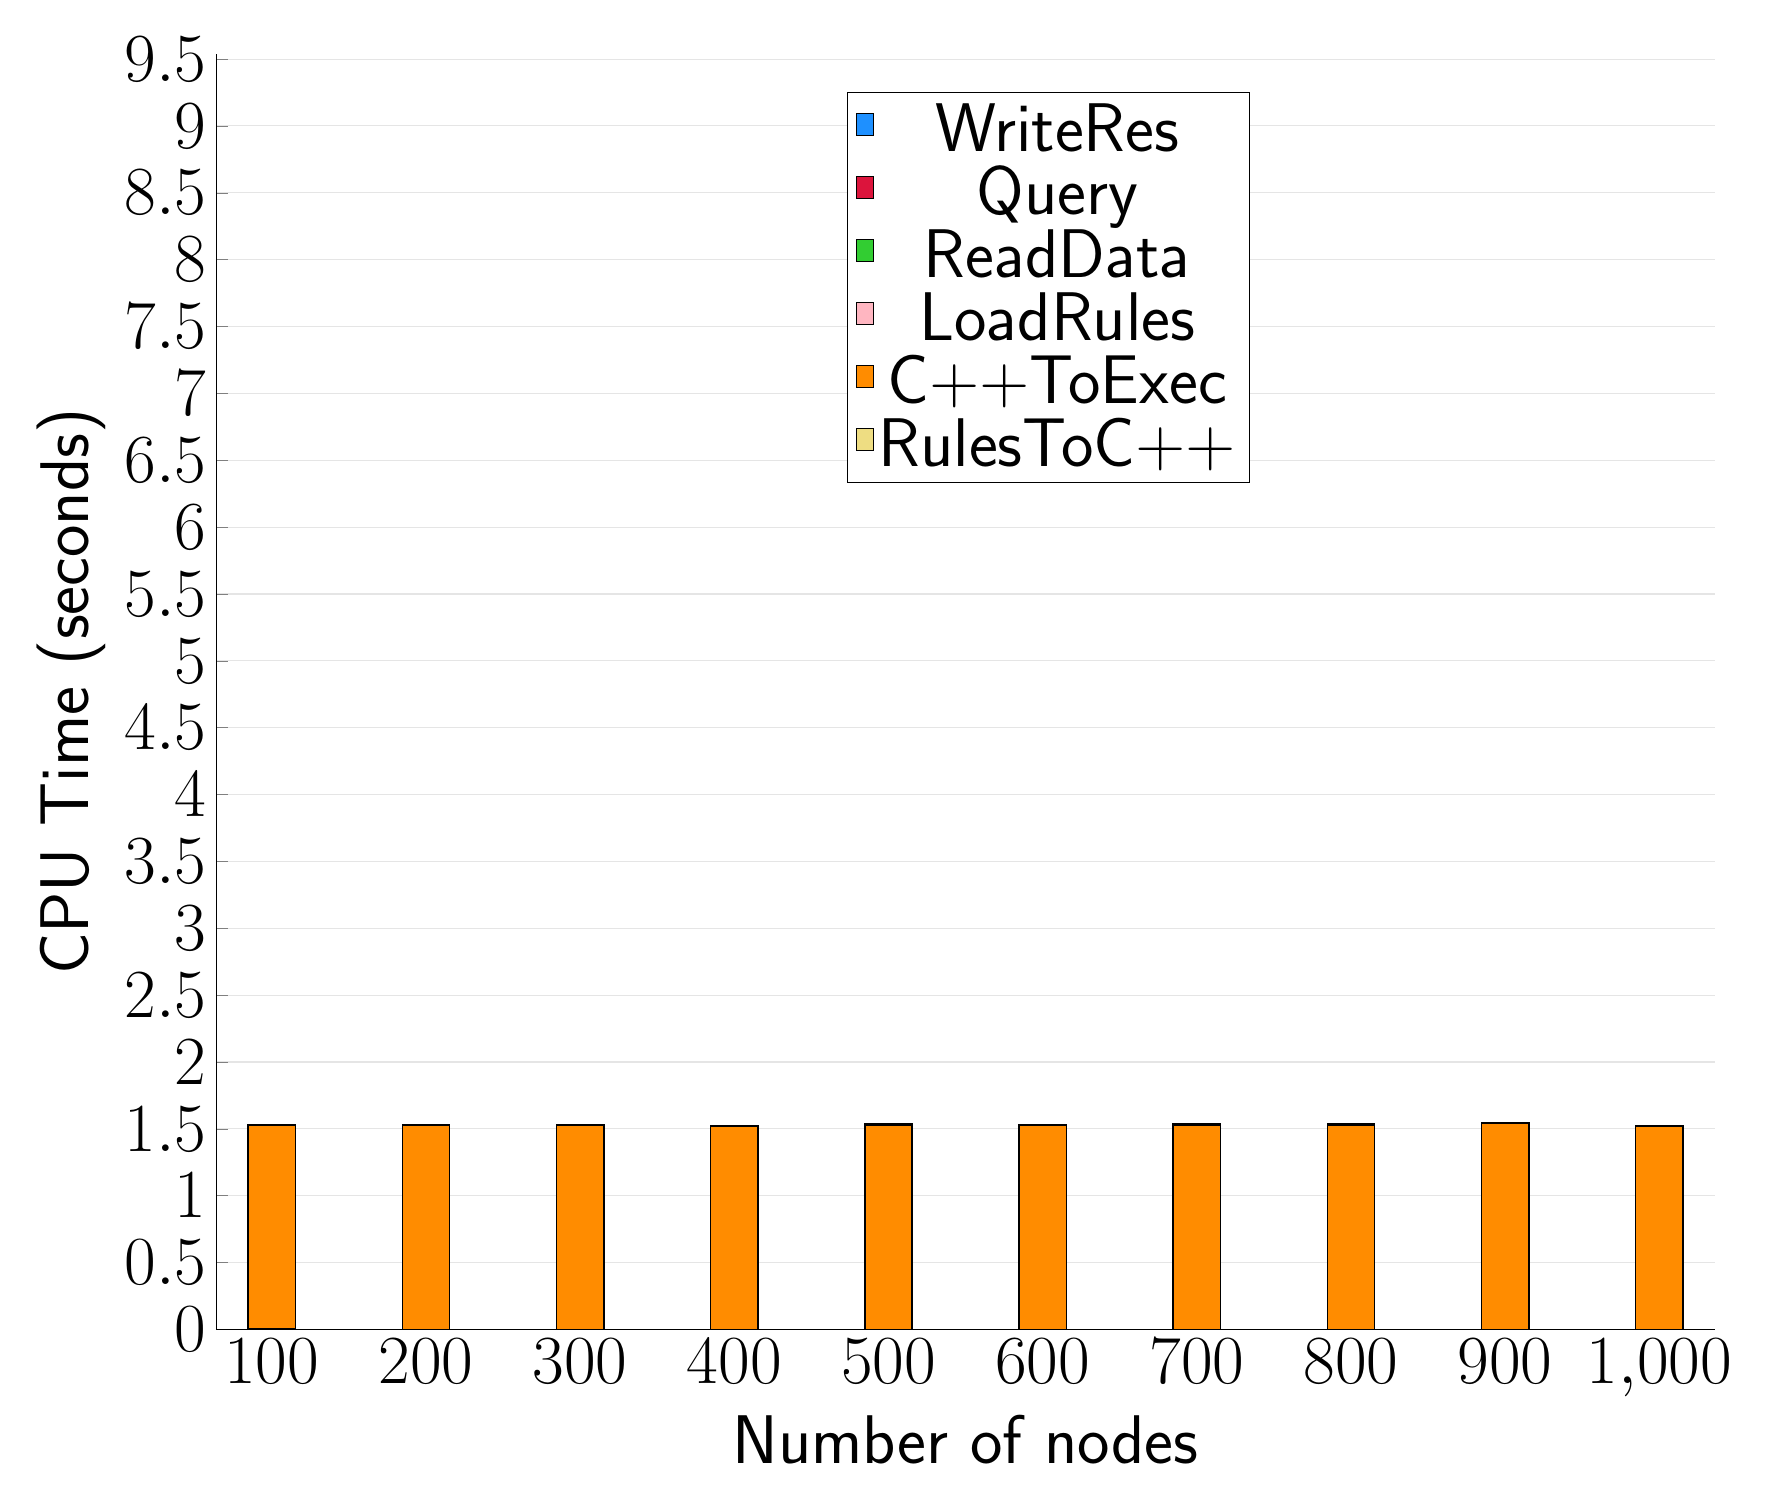
\begin{tikzpicture}
\begin{axis}[
   ybar stacked,
   width=1.7\textwidth,
   bar width=0.6cm,
   ymajorgrids, tick align=inside,
   major grid style={draw=gray!20},
   xtick=data,
   ymin=0, ymax=9.538,
   axis x line*=bottom,
   axis y line*=left,
   enlarge x limits=0.04,
   legend style={
       at={(0.69, 0.97)},
       anchor=north east,
       legend columns=1,
       font=\Huge,
   },
   ylabel={CPU Time (seconds)},
   xlabel={Number of nodes},
   label style={font=\Huge},
   tick label style={font=\Huge},
]
\addlegendimage{fill=DodgerBlue, draw=black, line width=0.2pt}
\addlegendentry{WriteRes}
\addlegendimage{fill=Crimson, draw=black, line width=0.2pt}
\addlegendentry{Query}
\addlegendimage{fill=LimeGreen, draw=black, line width=0.2pt}
\addlegendentry{ReadData}
\addlegendimage{fill=LightPink, draw=black, line width=0.2pt}
\addlegendentry{LoadRules}
\addlegendimage{fill=DarkOrange, draw=black, line width=0.2pt}
\addlegendentry{C++ToExec}
\addlegendimage{fill=LightGoldenrod, draw=black, line width=0.2pt}
\addlegendentry{RulesToC++}
\addplot +[fill=LightGoldenrod, draw=black, line width=0.55pt] coordinates {
(100, 0.0020000000000000005)
(200, 0.0)
(300, 0.0)
(400, 0.0)
(500, 0.0)
(600, 0.0)
(700, 0.0)
(800, 0.0)
(900, 0.0)
(1000, 0.0)
};
\addplot +[fill=DarkOrange, draw=black, line width=0.55pt] coordinates {
(100, 1.5260000000000002)
(200, 1.5259999999999998)
(300, 1.528)
(400, 1.5219999999999998)
(500, 1.53)
(600, 1.5260000000000002)
(700, 1.53)
(800, 1.53)
(900, 1.5380000000000003)
(1000, 1.5180000000000002)
};
\addplot +[fill=LightPink, draw=black, line width=0.55pt] coordinates {
(100, 0.0001676)
(200, 0.0001554)
(300, 0.0001538)
(400, 0.00015639999999999998)
(500, 0.0001622)
(600, 0.0001638)
(700, 0.00016159999999999997)
(800, 0.0001656)
(900, 0.0001702)
(1000, 0.0001716)
};
\addplot +[fill=LimeGreen, draw=black, line width=0.55pt] coordinates {
(100, 0.0008572)
(200, 0.0012242000000000002)
(300, 0.0015966)
(400, 0.0020156)
(500, 0.0023883999999999997)
(600, 0.002677)
(700, 0.0027954000000000004)
(800, 0.0032592000000000003)
(900, 0.0036856)
(1000, 0.0038528)
};
\addplot +[fill=Crimson, draw=black, line width=0.55pt] coordinates {
(100, 0.0002878)
(200, 0.000504)
(300, 0.0007999999999999998)
(400, 0.0010274)
(500, 0.0013440000000000001)
(600, 0.0015141999999999998)
(700, 0.0017112000000000002)
(800, 0.0019182000000000001)
(900, 0.002146)
(1000, 0.0024248)
};
\addplot +[fill=DodgerBlue, draw=black, line width=0.55pt] coordinates {
(100, 0.0001716)
(200, 0.00016620000000000003)
(300, 0.0002448)
(400, 0.00023580000000000004)
(500, 0.0002182)
(600, 0.0002382)
(700, 0.0002568)
(800, 0.0002232)
(900, 0.00021879999999999998)
(1000, 0.0001748)
};
\end{axis}
\end{tikzpicture}

\end{document}
